%-------------------------------------------------------------------------------------------------------
%
%
%
%-------------------------------------------------------------------------------------------------------    
\chapter{General Concepts}

At a higher level, the layout control system consists of components and a communication scheme. This chapter will define the key concepts of a layout system. At the heart of the layout control system is a common communication bus to which all modules connect. The others key elements are node, events, ports and attributes. Let's define these items first and then talk about how they interact. The following figure depicts the high level view of a layout control system.

\begin{figure}[h]
    \centering
    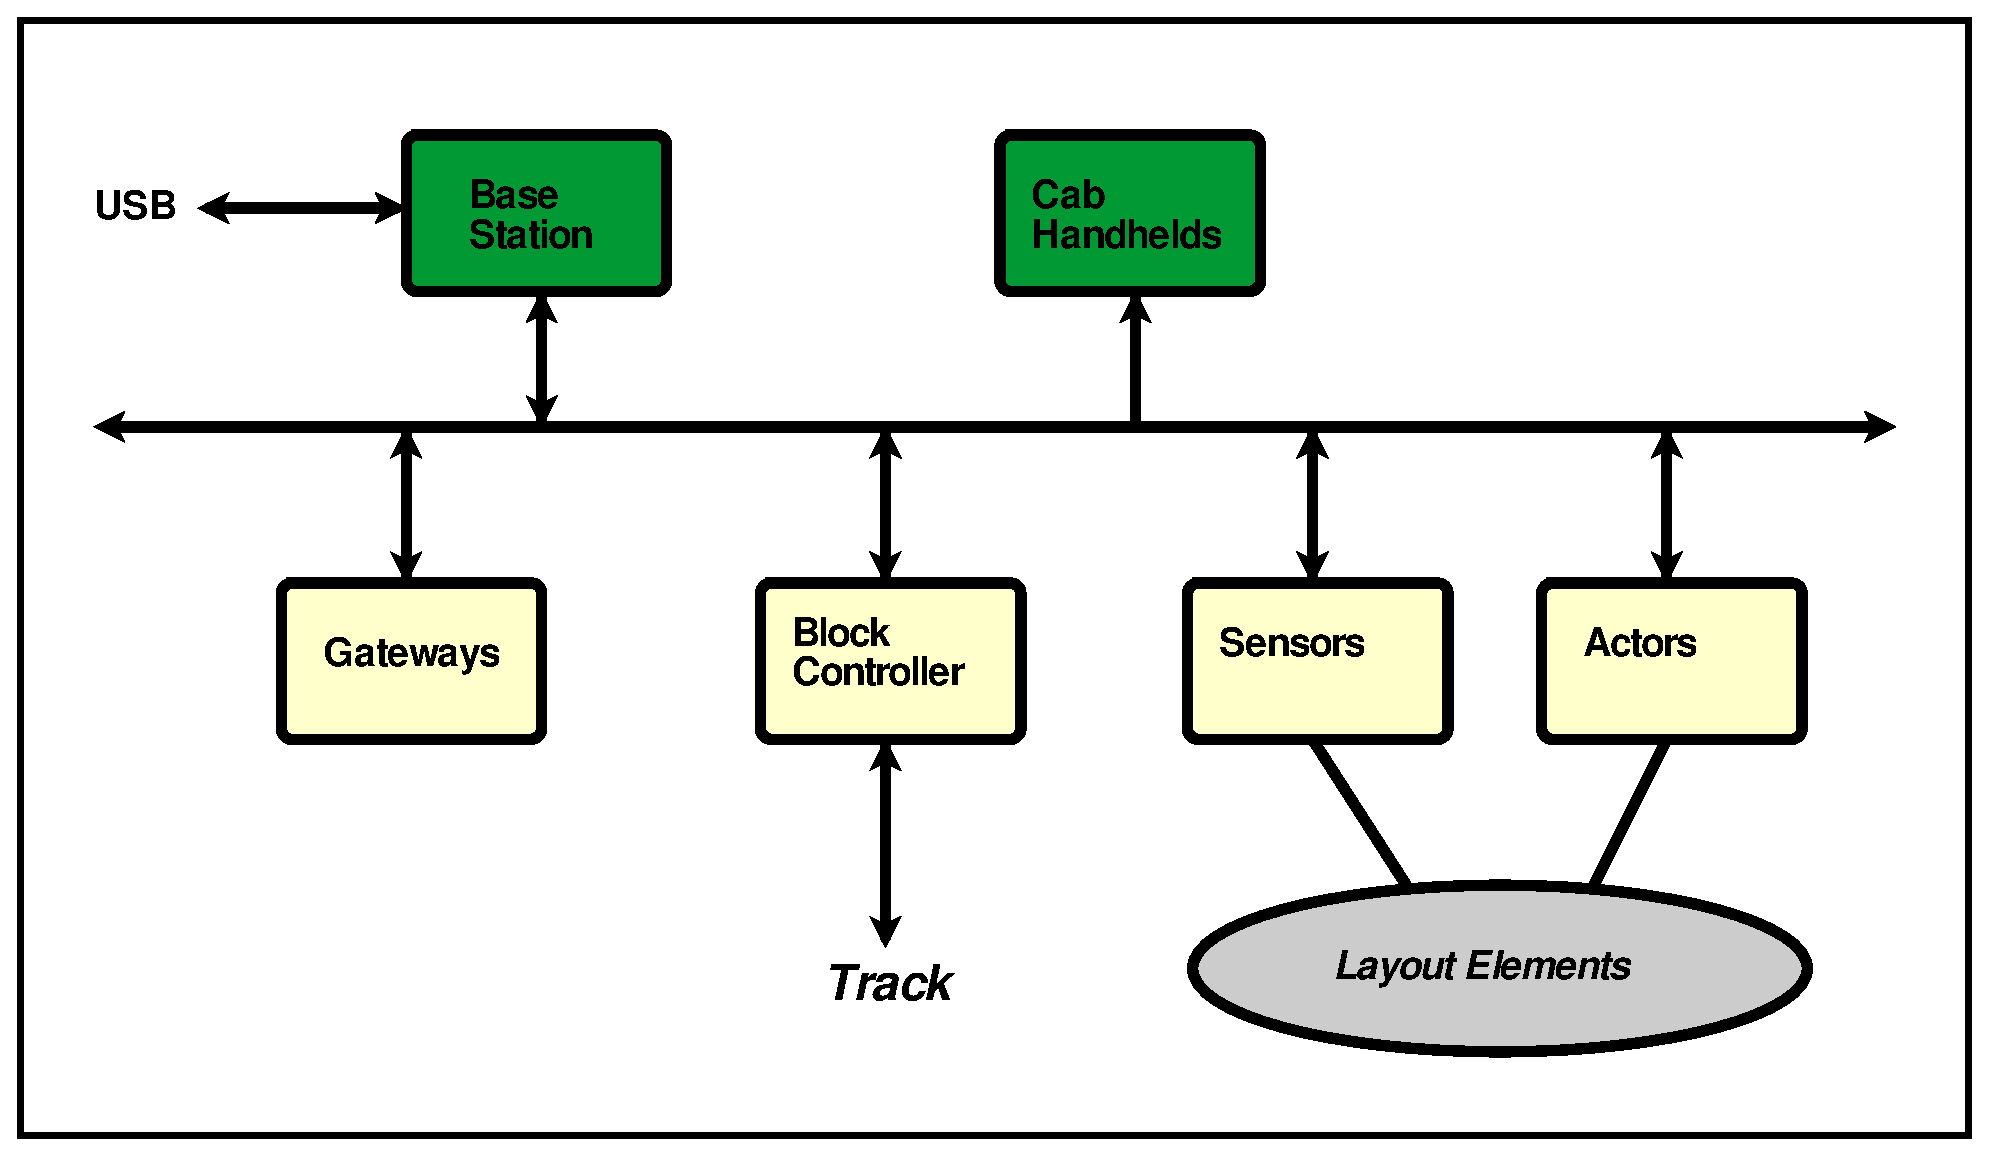
\includegraphics[page=1, width=\textwidth]{./figures/Schematic_LcsNodes-Layout-Overview.pdf}
\end{figure}

\section{Layout Control Bus}

The layout control bus is the backbone of the entire system. The current implementation is using the industry standard CAN bus. All hardware modules connect to this bus and communicate via messages. All messages are broadcasted and received by all other hardware modules on the bus. The classic CAN bus standard limits the message size to 8 bytes and this is therefore the maximum message size chosen for the LCS bus. The CAN bus also has a hardware module limit of about 110 modules for bandwidth reasons. But even for a large layout this should be sufficient. And for really large layouts, another bus system or a system with CAN bus routers, could be envisioned. The software should therefore be designed to manage thousands of connected modules. While the CAN bus technology could be exchanged, the message format and size defined as well as the broadcasting paradigm are fixed in the overall design and will not change.

\section{Hardware Module}

Everything connected to the LCS bus is a {\bf hardware module}, which is the physical entity connected to the bus. Typically it is a micro controller with the bus interface and hardware designed for the specific purpose. For example, a CAN bus interface, an AtMega Controller, and digital output drivers could form a hardware module to control railroad turnouts and signals. Base stations, handhelds and gateways are further examples of a hardware module. Hardware modules are expected to be physically located near their use and thus spread throughout the layout. Some hardware modules could be at locations that cannot be reached easily. So all interaction for configuration and operations needs to be possible through the messages on the bus. Nevertheless, putting local controls on a hardware module should not be prohibited.

A hardware module consists of a controller part and a node specific part. The controller part is the {\bf main controller}, which consists of the controller chip, a non-volatile memory to retain any data across power down, a CAN bus interface and interfaces to the node specific hardware. The node specific hardware is called the {\bf node extension}. Conceptually, both parts can be one monolithic implementation on one PCB board, but also two separate units connected by the extension connector. The are defined connectors between the boards. The hardware chapter will go into more detail on the board layouts and hardware design options.

\section{Nodes}

A hardware module is the physical implementation. A {\bf node} is the software entity running in the firmware of the hardware module. Nodes are the processing elements for the layout. Conceptually, a hardware module can host more than one node. The current implementation however supports only one node on a given hardware module. A node is uniquely identified through the {\bf node identifier}. There are two ways to set a nodeId. The first is to have central component to assign these numbers on request. The second method sets the number manually. Although a producer consumer scheme would not need a nodeId, there are many operations that are easier to configure when explicitly talking to a particular node. Both nodes and event identifiers are just numbers with no further classification scheme. A configuration system is expected to provide a classification grouping of nodes and event number ranges if needed.

A node also has a {\bf node type}, to identify what the node is capable of. Examples of nodes types are the base station, a booster, a switch module, a signal control module, and so on. While the node number is determined at startup time and can change, the node type is set via the module firmware. As the node type describes what the hardware module can do the type cannot change unless the module changes. Once the node has an assigned node number, configuration tools can configure the node via configuration messages to set the respective node variables.

A node needs to be configured and remember its configuration. For this purpose, each node contains a {\bf node map} that keeps all the information about the node, such as the number of ports, the node unique Id and so on. There is also a small set of user definable attributes to set data in a node map specific to the node. The data is stored in non-volatile memory space and on power up the node map is used to configure the node. If the module is a new module, or a module previously used in another layout, or the firmware version requires a new data layout of the node map, there is a mechanism to assign a new node number and initialize the node map with default values.

\section{Ports}

A node has a set of receiving targets, called ports. Ports connect the hardware world to the software world, and are the connection endpoints for events and actions. For example, a turnout digital signal output could be represented to the software as a port on a node. The node registers its interest in the event that target the signal. An event sent to the node and port combination then triggers a callback to the node firmware to handle the incoming events. Although a node can broadcast an event anytime by just sending the corresponding message, the event to send is typically associated with an outbound port for configuration purposes. In addition to the event immediate processing, the event handling can be associated with a timer delay value. On event reception the timer value will delay the event callback invocation or broadcast.

A node has a {\bf port map} that contains one entry for each defined port. {\bf port map entries} describe the configuration attributes and state of the port such as the port type. There is also a small set of user definable attributes to set data in a port map entry specific to the port. These attributes can be used by the firmware programmer to store port specific data items such as a hardware pin or a limit value in the port map.

\section{Attributes}

{\bf Node attributes} and {\bf port attributes} are conceptually similar to the CV resources in a DCC decoder. Many decoders, including the DCC subsystem decoders, feature a set of variables that can be queried or set. The LCS layout system implements a slightly different scheme based on items. In contrast to a purely decoder variable scheme an item can also just represent just an action such as setting an output signal. Items are passed parameter data to further qualify the item. Items are just numbers assigned. The range of item numbers is divided into a reserved section for the layout system itself, and a user defined range that allows for a great flexibility to implement the functions on a particular node and port. The meaning of user defined items is entirely up to the firmware programmer. If it is desired to have a variables, a combination of items and attributes can provide the traditional scheme as well. In addition, there are node local variables, called attributes, available to the firmware programmer for storing data items.

\section{Events}

The LCS message bus, hardware module, node and ports describe layout and are statically configured. For nodes to interact, {\bf events} and their configuration is necessary. An event is a message that a node will broadcast via the bus. Every other node on this bus will receive the event and if interested act on the event. The sender is the producer, the receiver is the consumer. Many producers can produce the same event, many consumers can act on the same event. The {\bf event Id}, a 16 bit number, is unique across the layout and assigned by a configuration tool during the configuration process. Other than being unique, there is no special meaning, the number is arbitrary. There are in total 65536 events available.

In addition to the event Id, an event message contains the node Id of the sender. While most events will be an ON/OFF event, events can also have additional data. For example an overload event sent by a booster node, could send the actual current consumption value in the event message. A consumer node registers its interest in an event by being configured to react to this event on a specific port. The node maintains an {\bf event map}, which contains one entry for each event id / port id combination. For the eventing system to work, the nodeID is not required. Any port on any node can react to an event, any node can broadcast an event.

To connect producers to consumers, both parties need to be told what to do with a defined event. A producer node outbound port needs to be told what event to send for a given sensor observation. For example, a simple front panel push button needs to be told what event to send when pushed. Likewise, a consumer node inbound port needs to be told what events it is interested in and what the port should do when this event is received. Both meet through the event number used. While an inbound port can be configured to listen to many event Ids, an outbound port will exactly broadcast one eventId.

Any port on any node can react to an event, any node can broadcast an event. Still, addressing a node and port combination explicitly is required for two reasons. The first is of course the configuration of the node and port attributes. Configuration data needs to go directly to the specified node and port. The second reason is for directly accessing a resource on the layout. For example, directly setting a turnout connected to one node. While this could also be implemented with associated an event to send when operating a turnout, it has shown beneficial and easier to configure also directly access such a resource through a dedicated node/port address.

\section{DCC Subsystem}

The node, ports and events are the foundation for building a layout system based on the producer / consumer scheme. The scheme will be used heavily for implementing turnout control, signals, signal blocks and so on. In addition, there is the management of the mobile equipment, i.e. locomotives. The DCC subsystem is the other big part of our layout control system. In a sense it is another bus represented by the track sections.

LCS messages for DCC commands are broadcasted from controlling devices. For example, a handheld broadcasts a speed setting DCC command. In a layout there is one base station node which is responsible to produce the DCC signals for the track. The DCC signals are part of the physical LCS bus. While a base station design could directly supply the signal current to the track, larger layouts will typically have one or more boosters. They take the DCC signal from the LCS bus lines and generate the DCC signal current for their track section. All LCS messages for DCC operations are broadcasting messages, all nodes can send them, all nodes can receive them. Handhelds, base station and boosters are thus just nodes on the LCS bus. Only the base station will however generate the DCC signal.

The DCC standard defines mobile and stationary decoders. The DCC signal could also be used to control for example a set of turnouts via a stationary decoder. The LCS DCC  message set contains messages for addressing a stationary decoder. Since the commands for stationary equipment are just DCC commands, they will be transmitted via the track as well and take away bandwidth on the track. A layout will therefore more likely use the LCS bus for implementing the management of stationary equipment. Besides, the producer / consumer model allows for a much greater flexibility when building larger and partially automated layouts.

\section{Analog Subsystem}

The layout control system is primarily a digital control system. There are however layout use cases where there are many analog locomotives that would represent a significant investment when converting to DCC or that cannot easily be equipped with a DCC decoder. In a DCC subsystem the decoder is in the locomotive and many locomotives can run therefore on the same track. In an analog system, the locomotive has no capabilities and therefore the track needs to be divided into sections that can be controlled individually. One locomotive per section is the condition. In a sense the decoder becomes part of the track section. The layout control system offers support for building such a track section subsystem. Often the sections are combined into blocks and build the foundation for a block signaling system. Note that the rest of the layout control system is of course digital. What is typically the booster to support a section of track, is the block controller for an analog layout. We will see in the later chapters that booster and block controller are very similar and design a block controller to accommodate both use cases.

\section{Configuration Mode}

Before operations the nodes, ports and events need to be configured. Once a node has an assigned valid nodeId, the node configuration is the process of configuring a node global information, the event map information and the finally the port information. The information is backed by non-volatile storage, such that there is a consistent state upon node power up. During operations, these value can of course change, but are always reset to the initial value upon startup.

The primary process of configuration is inventing events numbers and assigning them producers and consumers. The process follows the general "if this then that" principle. On the producer side the configuration process assigns a port to an event, i.e. the push of a button to an event to send. If this button is pushed then send that event. On the consumer side the configuration process is to assign the event to a port. If this event is received then execute that port action.

After the node is up and running with a valid node Id, there are event configuration messages than can be send to the node to set the event mapping table with this information. The event map table is the mapping between the event and the port associated. Events are thus configured by "teaching" the target node what port to inform about an occurring event.

\section{Operation Mode}

Besides the basic producer/consumer model with the event messages as communication mechanism, there are several LCS control and info messages used for managing the overall layout with signals turnouts and so on as well as the physical track and the running equipment. In a layout, the track typically consist of one or more sections, each managed by a booster or block controller node. Track sections are monitored for their power consumption to detect short circuits. Back communication channels such as RailCom are handled by the booster node and provide information about the running equipment. Stationary equipment such as turnouts and signals as well as detectors, such as track occupancy detectors or turnout setting detectors are monitored and controlled through LCS messages and the event system. Conceptually any node can send and receive such event, info or control messages. Some nodes, however have a special role.

For example, the key module for layout operations is the {\bf base station}. The base station, a node itself, is primarily responsible for managing the active locomotives on the layout. When a control handheld wants to run a locomotive, a cab session for that locomotive is established by the base station. Within the session, the locomotive speed, direction and functions are controlled through the cab handheld sending the respective messages. The base station is responsible for generating the DCC packets that are sent by the booster or block controller power module to the actual track sections. Booster and block controller module are - you guessed it - node themselves.

Finally, there are LCS nodes that represent cab handhelds to control a locomotive or consists, layout panel connectors, gateways to other layout protocols, sensors and actors to implement for example turnout control, signaling, section occupancy detections and many more. All these components share the common LCS bus and use ports and events to implement the capabilities for operating a layout.

In a layout with many track sections the {\bf block controller} is a special node that will manage a block on the layout. Like all other nodes, a block controller itself is a node that can react to events and is controller and monitored by LCS messages. There will be several chapters devoted to this topic later.

\section{Summary}

This chapter introduced the basic concepts of the layout control system described in this book. It follows very few overall guiding principles. Above all, there is the clear separation of what needs to be available for operating the mobile equipments, i.e. locomotives, and the stationary layout elements. Controlling mobile decoders are left to the DCC subsystem, all other communication takes place via the LCS bus, which is the bus to which all of the hardware modules connect. Hardware modules host the nodes. Currently, a hardware module hosts exactly one node. A node can contains one or many ports, which are the endpoints for the event system. There is a set of user allocated attributes available to node and ports. Node, port and attribute data are backed by non-volatile memory, so that a restart will use defined initial values. Nodes and their ports are also directly addressable, which is needed for configuration purposes and the directly addressable components model. Using the producer / consumer paradigm, sensors generate events and interested actors just act on them. The configuration process is simply to assign the same event to the producer node and consumer node / port id when they should work together.

The communication bus should rest on a reliable bus with a sufficient bandwidth. Although the CAN bus is used in the initial implementation, it is just one option and other technologies can be considered. In all cases however, the message format should be available for a variety of bus technologies. Our messages are therefore short, up to eight data bytes. This causes on the one hand some complexity for data items larger than a few bytes on the other hand no messages blocks the bus for a longer period. The bus technology is expected to reliably deliver a message but does not ensure its processing. This must be ensured through a request reply message scheme built on top.

